
%=============================================================================
% ... THIS IS chapter{ESDRU: Energy-based Spatial Distortion Reference Unit} ...
% Revisions
% Dec.2021 - First version
%=============================================================================
%=============================================================================
\chapter{ESDRU: Energy-based Spatial Distortion Reference Unit}
%=============================================================================

\section{Introduction}

Subjective listening tests benefit from having known quality references within
the listening test material. For P.800 monaural listening tests, the MNRU has
been widely adopted. Another example is ITU-R Rec. BS.1534, where the anchor condition(s)
are formed using a low pass filter. For testing stereo conditions, e.g. within
P.811, it is beneficial to have the reference condition include the stereo or 
spatial dimension. P.811 outlines two variants of a spatial distortion reference
unit (SDRU). Here, the ESDRU variant is described.



\section{Description of the Algorithm}

An overview of the algorithm can be found in P.811 \cite{P.811}. The basis for
the modulation is the same as for the SDRU \cite{P.811}, and can be described by
the equation

  \[
    \left\{
       \begin{array}{ll}
         {SDRU}_L(n) = g_4(n) \left( \alpha Ch_L(n)+(1-\alpha)Ch_R(n) \right) \\
         {SDRU}_R(n) = g_5(n) \left( \alpha Ch_R(n)+(1-\alpha)Ch_L(n) \right) \\
       \end{array}
     \right.
  \]

where $n$ is the sample index and $\alpha$ is the spatial degradation factor that
ranges between $[0,1.0]$. $g_4(n)$ and $g_5(n)$ are complementary gains from a
spatial modulation function where
 
  \[
    g_5(n) = 1 + \alpha - g_4(n),
  \]
  
meaning that $g_5(n)$ will be $1$ when $g_4(n)$ is $\alpha$ and $g_5(n)$ will be $\alpha$
 when $g_4(n)$ is $1$. The modulation function is what differs between the ESDRU and
\cite{SDRU}. For the latter, a triangular modulation function with a period of 1 second
is used. Here, the modulation is characterized by a step-wise random pattern. The function
that generates the modulation pattern is called g\_mod\_nrg.

{\tt\small
\begin{verbatim}
void g_mod_nrg(
    const double *input, /* i: Stereo input signal                 */
    const long length,   /* i: Length of input signal in samples   */
    const long step,     /* i: Length of transition in samples     */
    const double e_step, /* i: Energy step in high energy segments */
          double *m      /* o: Modulation curve                    */
)
\end{verbatim}
}

The \texttt{input} is the interleaved stereo signal read from file, \texttt{length} is the number
of samples, \texttt{step} is the interval where new values of the modulation is considered and also
the number of samples in the transition, and \texttt{e\_step} is the allowed step size during high-energy
segments. High-energy segments of the input signal are defined as when the short-term energy estimate 
$e_s(n)$ is above the long-term energy estimate $e_l(n)$. The energy of the input signal is first computed
by the function \texttt{energy}.

{\tt\small
\begin{verbatim}
/*-------------------------------------------------
 * Compute energy of left + right
 * e( n ) = left( n ).^2 + right( n ).^2
 *-------------------------------------------------*/
void energy(
    const double *input,  /* i: Input signal       */
    double *e,            /* i: Output signal      */
    const long length     /* i: Length of signal   */
)
{
    long i;
    for( i = 0; i < length; i++ )
    {
        e[i] = input[2 * i] * input[2 * i] + input[2 * i + 1] * input[2 * i + 1];
    }

    return;
} 
\end{verbatim}
}

The short-term and long-term energy envelopes are derived by applying a one-pole first order IIR-filter
of the form:

  \[
    y(n) = \beta x(n) + (1 - \beta) y(n-1)
  \]

where $\beta$ is the low-pass filtering factor. The filtering is applied in forward and reversed time order
on for both $e_s(n)$ and $e_l(n)$ to get a symmetric filtering of the energy values. This is implemented using
the function \texttt{ar1}, where the last argument controls forward (1) or backward (-1) time order. Finally,
a scaling of 0.77813 is applied to the long-term envelope $e_l(n)$ to lower it relative to short-term envelope 
$e_s(n)$. 

{\tt\small
\begin{verbatim}
    ar1( 0.001, e, es, length, -1 );
    ar1( 0.001, es, es, length, 1 );
    ar1( 0.0001, es, el, length, -1 );
    ar1( 0.0001, el, el, length, 1 );
    scale( el, 0.77813, el, length );
\end{verbatim}
}

The same operation may also be written in MATLAB code as follows:

{\tt\small
\begin{verbatim}
% Short-term energy envelope
alpha1 = 0.001;
[B,A] = iir1(alpha1);
es = filter(B,A,flipud(filter(B,A,flipud(e))));

% Long-term energy envelope
alpha2 = 0.0001;
beta = 0.77813;
[B,A] = iir1(alpha2);
el = beta*filter(B,A,flipud(filter(B,A,flipud(es))));
\end{verbatim}
}

The modulation may change at a step size of 1.5 ms. At each change point, a new value is chosen
with a probability of 0.2. This is implemented by comparing a random number generator with 0.2. If the decision
is taken to change level, the next level is generated as a random number in the range $[0,1.0]$. Next, if
the current signal segment is considered to be a high-energy segment, the step towards the new random level is
scaled with \texttt{e\_step}, effectively limiting the step-size during high-energy segments. By default, 
\texttt{e\_step} is set to 0.5, which allows to go half-way to the new random level. If \texttt{e\_step} would
be set to zero, the modulation function would not change at all during high energy segments. Finally, if \texttt{e\_step}
would be set to 1, the step size would not be limited at all during high energy segments.

Once a new random value has been set, a cosine-shaped transition window is used to make a smooth transition to the
new value. The following code generates a modulation function $g\_mod\_nrg(n)$ in the range $[0,1.0]$. 

{\tt\small
\begin{verbatim}
    m_prev = 1.0;
    while( i < length )    
    {
        if( (rand() / ((double)RAND_MAX)) < 0.2 )
        { 
            if( es[i] < el[i] )
            {
                m_delta = 1.0;
            }
            else
            {
                m_delta = e_step;
            }
            m_new = rand() / ((double)RAND_MAX) * m_delta + m_prev * (1.0 - m_delta);
        }
        else
        {
            m_new = m_prev;
        }

        for(j = 0; j < step && i < length; i++,j++ )
        {
            xf_win = 0.5 * (1.0 - cos( LOCAL_PI * j / step ));
            m[i] = m_new * xf_win + m_prev * (1.0 - xf_win);
        }
        m_prev = m_new;
    }
\end{verbatim}
}    
    
The modulation functions $g_4(n)$ and $g_5(n)$ may then be derived from $g\_mod\_nrg(n)$ as 

  \[
    \left\{
       \begin{array}{ll}
            g_4(n) = 1.0 - g\_mod\_nrg(n) (1.0 - \alpha) \\
            g_5(n) = 1.0 + \alpha - g_4(n)               \\
       \end{array}
     \right.
  \]
  
Once the modulation function has been generated, the spatial distortion is applied using the 
function \texttt{apply\_spatial\_dist}.


\begin{figure}[htp]
    \begin{center}
        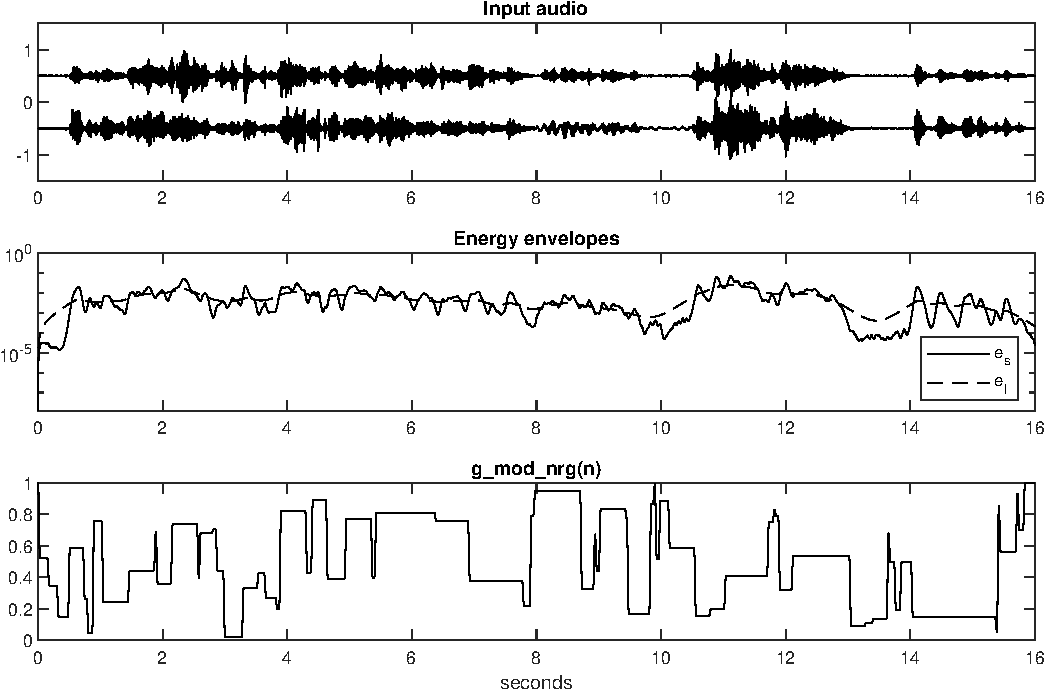
\includegraphics[scale=1.0]{esdru_spatial_modulation.pdf}
  \end{center}
  \caption{The energy of the input file is analyzed and then low-pass filtered to form a 
           short-term estimate $e_s(n)$ and a long-term estimate $e_l(n)$. When the short-term  
           estimate is above the long-term estimate, $e_s(n)>e_l(n)$, it is considered a high-energy
           segment and the change in modulation is limited by $e_{step}$.
           \label{fig:esdru_spatial_modulation} }
\end{figure}



\section{Usage of esdru}

{\tt\small
\begin{verbatim}
esdru [options] <alpha> <input file> <output file>

<alpha>           Alpha value [0.0 ... 1.0]
<input file>      Input file, 16 bit Stereo PCM
<output file>     Output file, 16 bit Stereo PCM

Options:
-sf FS            Sampling frequency FS Hz (Default: 48000 Hz)
-e_step S         Max step S during high energy [0.0 ... 1.0] (Default: 0.5)
-seed I           Set random seed I [unsigned int] (Default: 1)
\end{verbatim}
}
